\documentclass{beamer}
\usetheme{default}
\usepackage{booktabs}
\definecolor{mycolor1}{RGB}{17,29,74}
\definecolor{mycolor2}{RGB}{131,128,182}
\definecolor{mycolor3}{RGB}{194,202,232}

\setbeamercolor{title}{fg=mycolor1} 
\setbeamercolor{Huge}{fg=mycolor2} 
\setbeamercolor{frametitle}{fg=mycolor2} 
\setbeamercolor{subtitle}{fg=mycolor1} 

\setbeamercolor{itemize item}{fg=mycolor3} 
\setbeamercolor{enumerate item}{fg=mycolor3} 
\setbeamercolor{itemize item enumerate item}{fg=mycolor3} 
\usefonttheme{serif}
\usepackage{ragged2e}

\title[SkillVine]{\textbf{TrustFunds}}
\subtitle{\textit{A decentralised crowdfunding platform for empowering efficient fundraising.}}

\date{}
\begin{document}

{\usebackgroundtemplate{
\includegraphics[width=\paperwidth,height=\paperheight]{assets/image.png}}
\begin{frame}[plain]
  \vspace{60pt}
  \centering
  \maketitle
\end{frame}
}

{
\begin{frame}
  \frametitle{Team Members and Project Guide}
  \begin{itemize}
    \item Abraham V Shajan (KTE20CS004)
    \item Alvin Varghese (KTE20CS008)
    \item Amalia F (KTE20CS009)
    \item Aswin U S (KTE20CS019)
    \vspace{10pt}
    \item Project Guide: Prof. Nisha K K
  \end{itemize}
\end{frame}
}

\section{Introduction}
\begin{frame}
  \frametitle{Introduction}
  \begin{itemize}
    \item Decentralized Crowdfunding: Blockchain \& Smart Contracts.
    \vspace{10pt}
    \item Efficient, Secure, Autonomous, Transparent Fundraising.
    \vspace{10pt}
    \item Immutable Ledger for Trustworthy Transactions.
    \vspace{10pt}
  \end{itemize}
\end{frame}

\section{System Design}
    \begin{frame}{System Design}
        Web UI:
        \begin{itemize}
            \item Web UI - Responsive for both mobile and desktop screens.
            \item React js
            \item Connectivity and API Integration - Axios for request management.
            \end{itemize}
            \vspace{17pt}
        Server/API:
         \begin{itemize}
            \item RESTful API for data exchange in JSON Format.
            \item Node js
            \end{itemize}
    \end{frame}
    
    \begin{frame}{System Design}
   Database:
          \begin{itemize}
           \item NoSQL database for storing user, campaign related data.
           \item MongoDB
            \vspace{17pt}
        \end{itemize} 
    Blockchain Module:
           \begin{itemize}
             \item  Smart Contracts: Creating, managing, and finalizing crowdfunding campaigns.
             \item Web3.js: Communication between the front end and the Ethereum blockchain network.
             \end{itemize} 
    \end{frame}
    
\section{Sequence Diagrams}
\begin{frame}{Sequence Diagram}
    \hspace*{-1cm}
    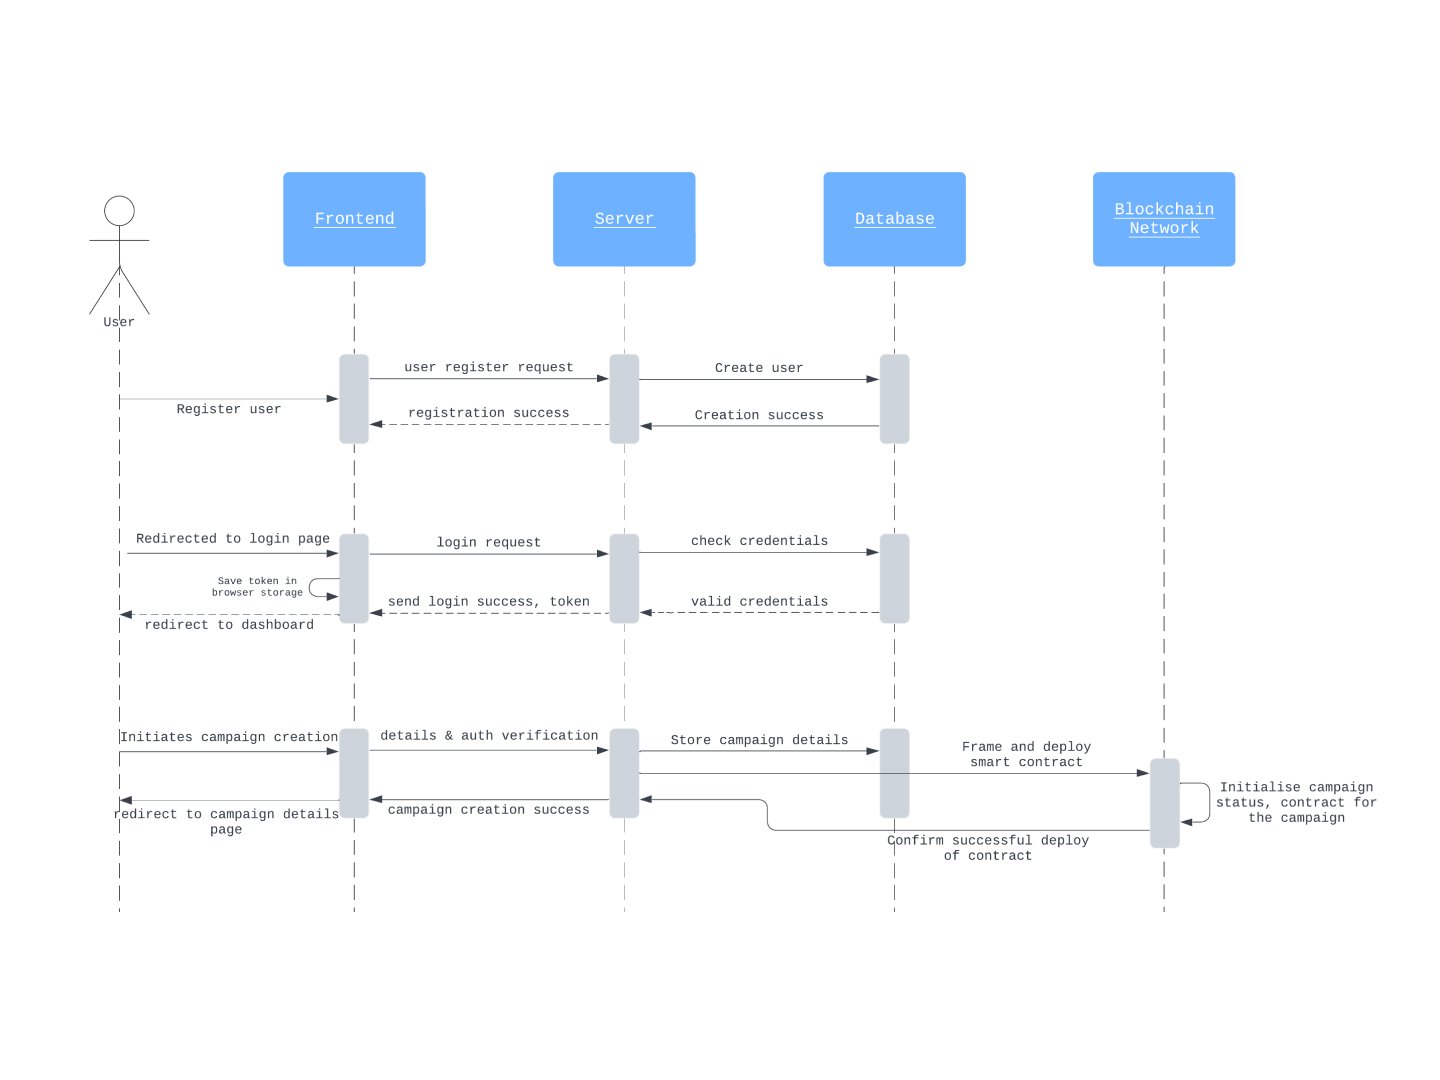
\includegraphics[width=360pt]{assets/seqdiags/seq1.png} 
\end{frame}
\begin{frame}{Sequence Diagram}
    \hspace*{-1cm}
    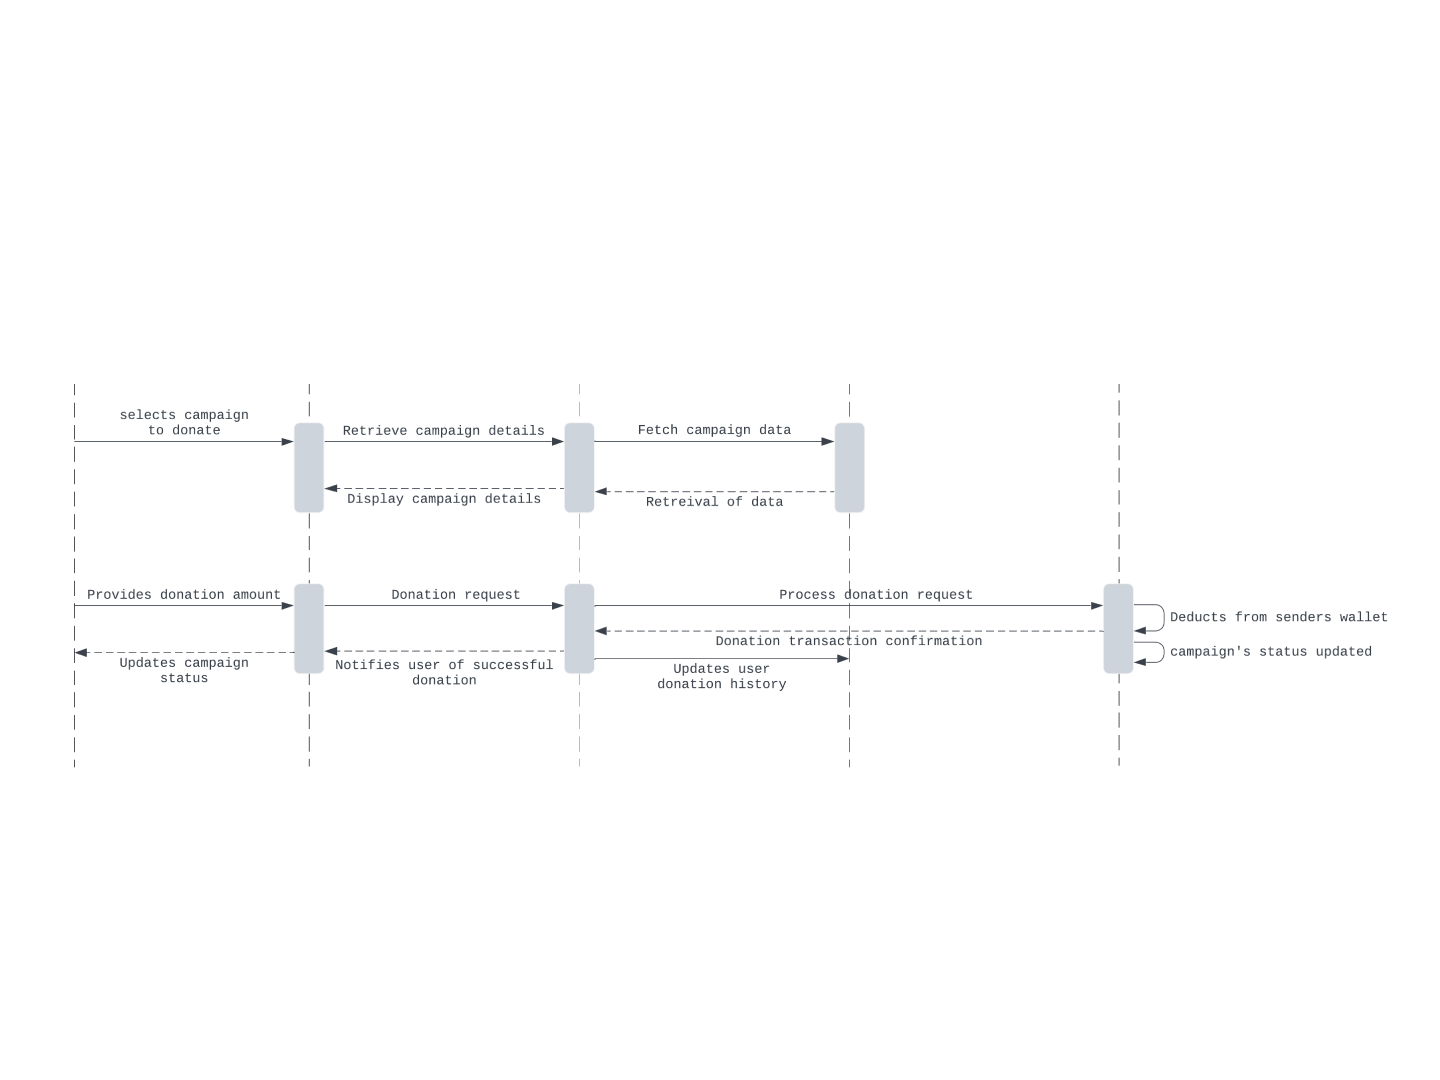
\includegraphics[width=360pt]{assets/seqdiags/seq2.png} 
\end{frame}
    
\section{UI}
\begin{frame}{Web UI - Register page}
    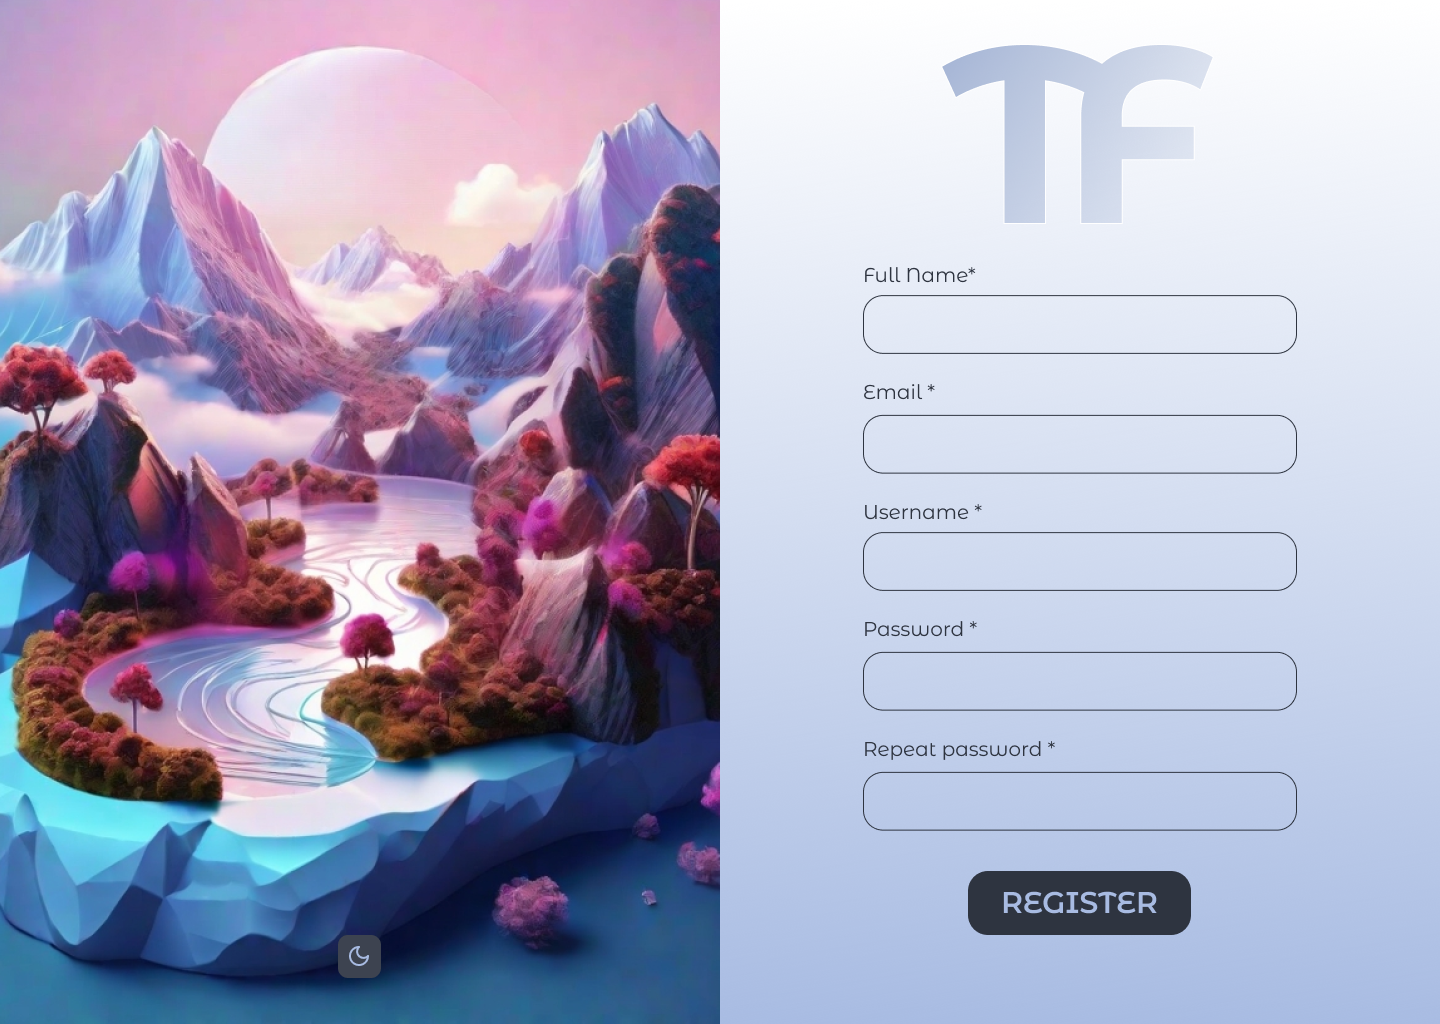
\includegraphics[width=\linewidth]{assets/ui/register-light.png} 
\end{frame}
\begin{frame}{Register page}
    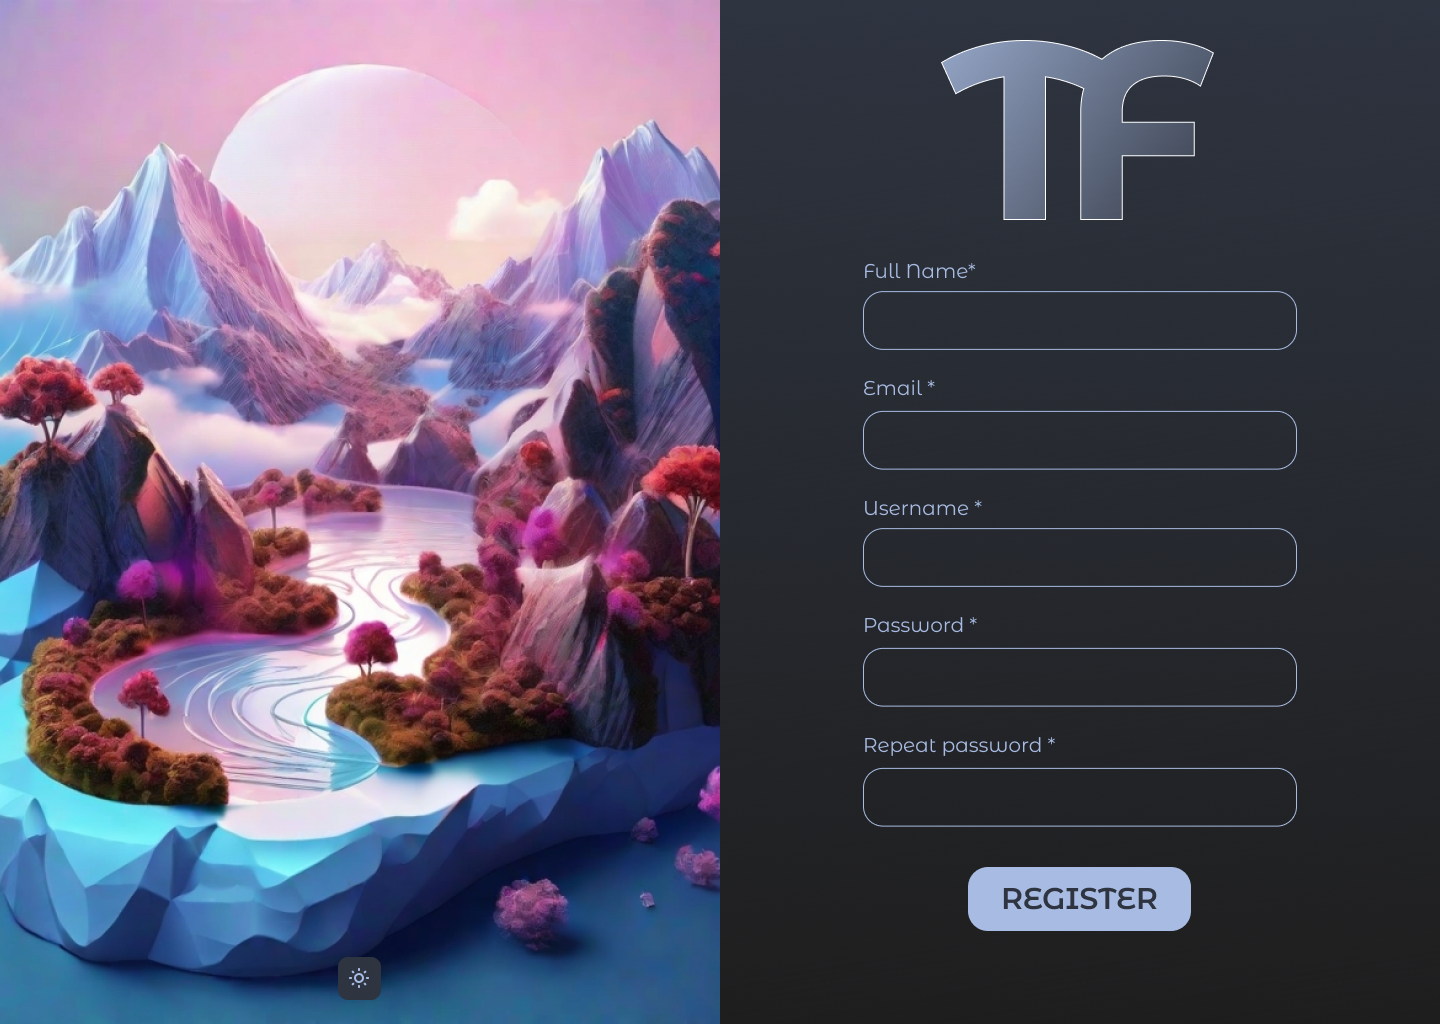
\includegraphics[width=\linewidth]{assets/ui/register.png} 
\end{frame}
\begin{frame}{Login page}
    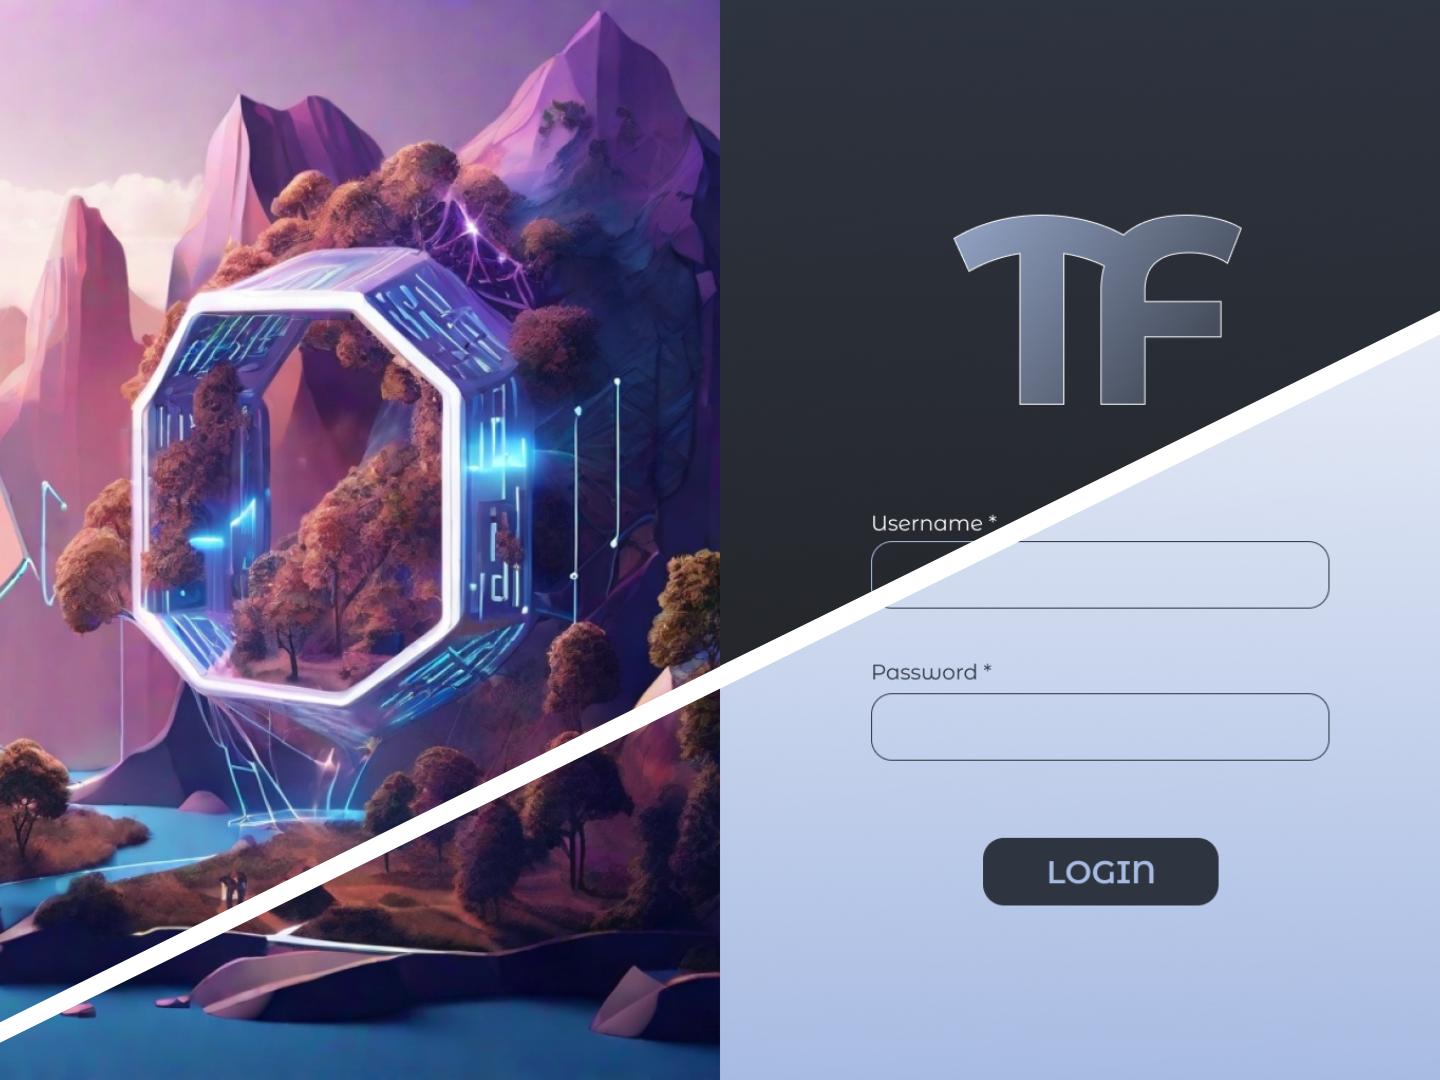
\includegraphics[width=\linewidth]{assets/ui/login.png} 
\end{frame}
\begin{frame}{Homepage}
    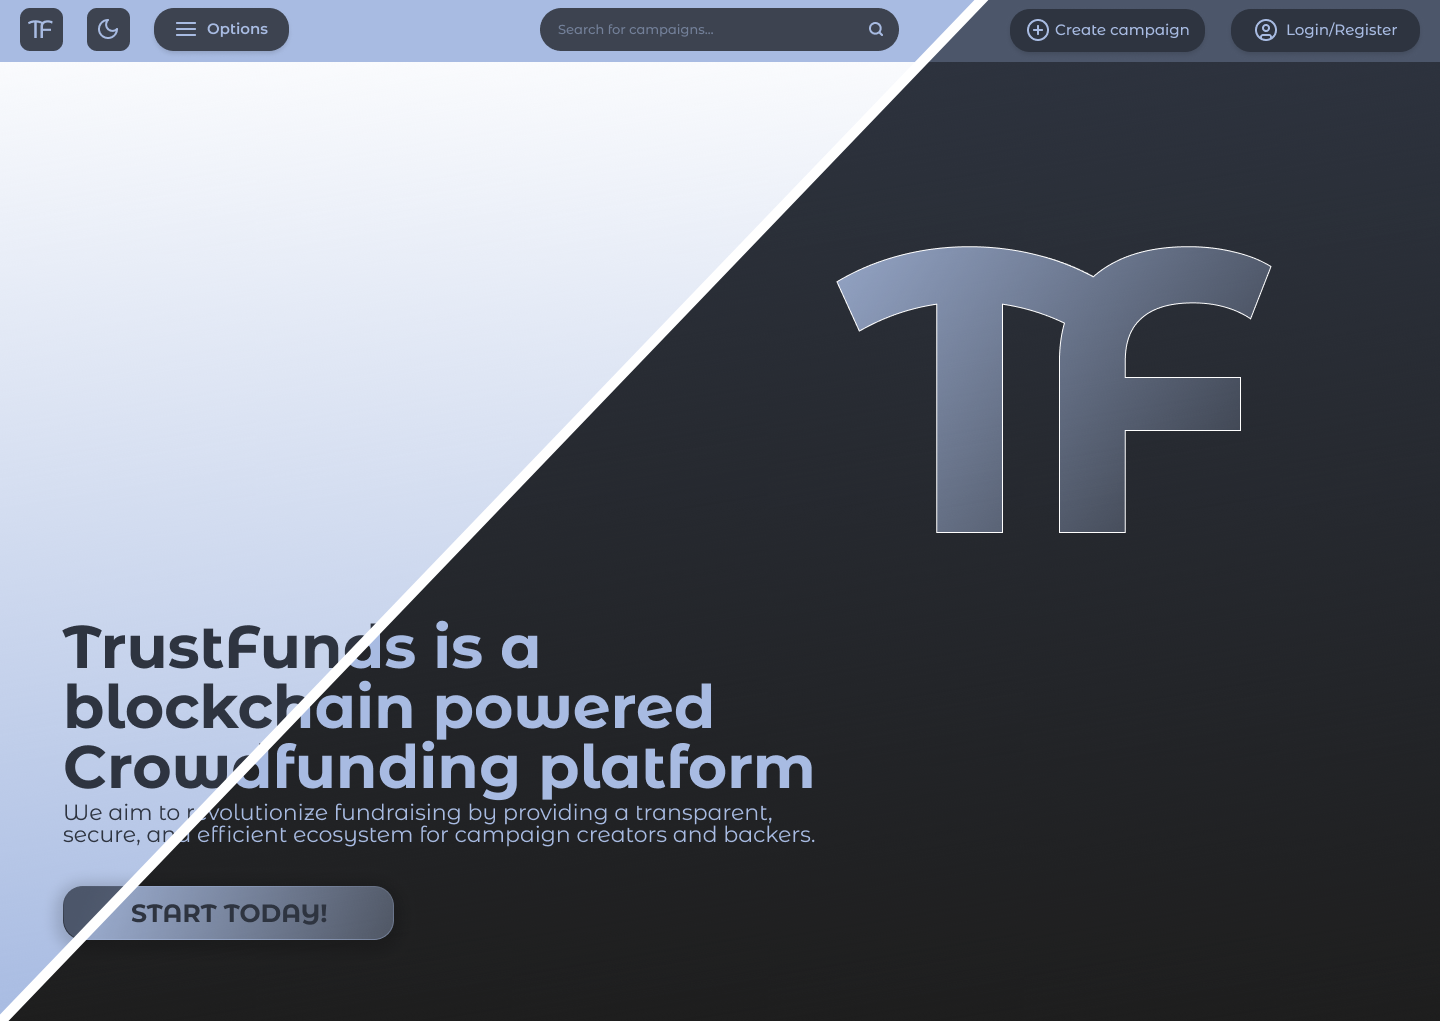
\includegraphics[width=\linewidth]{assets/ui/homepage.png} 
\end{frame}
\begin{frame}{Dashboard}
    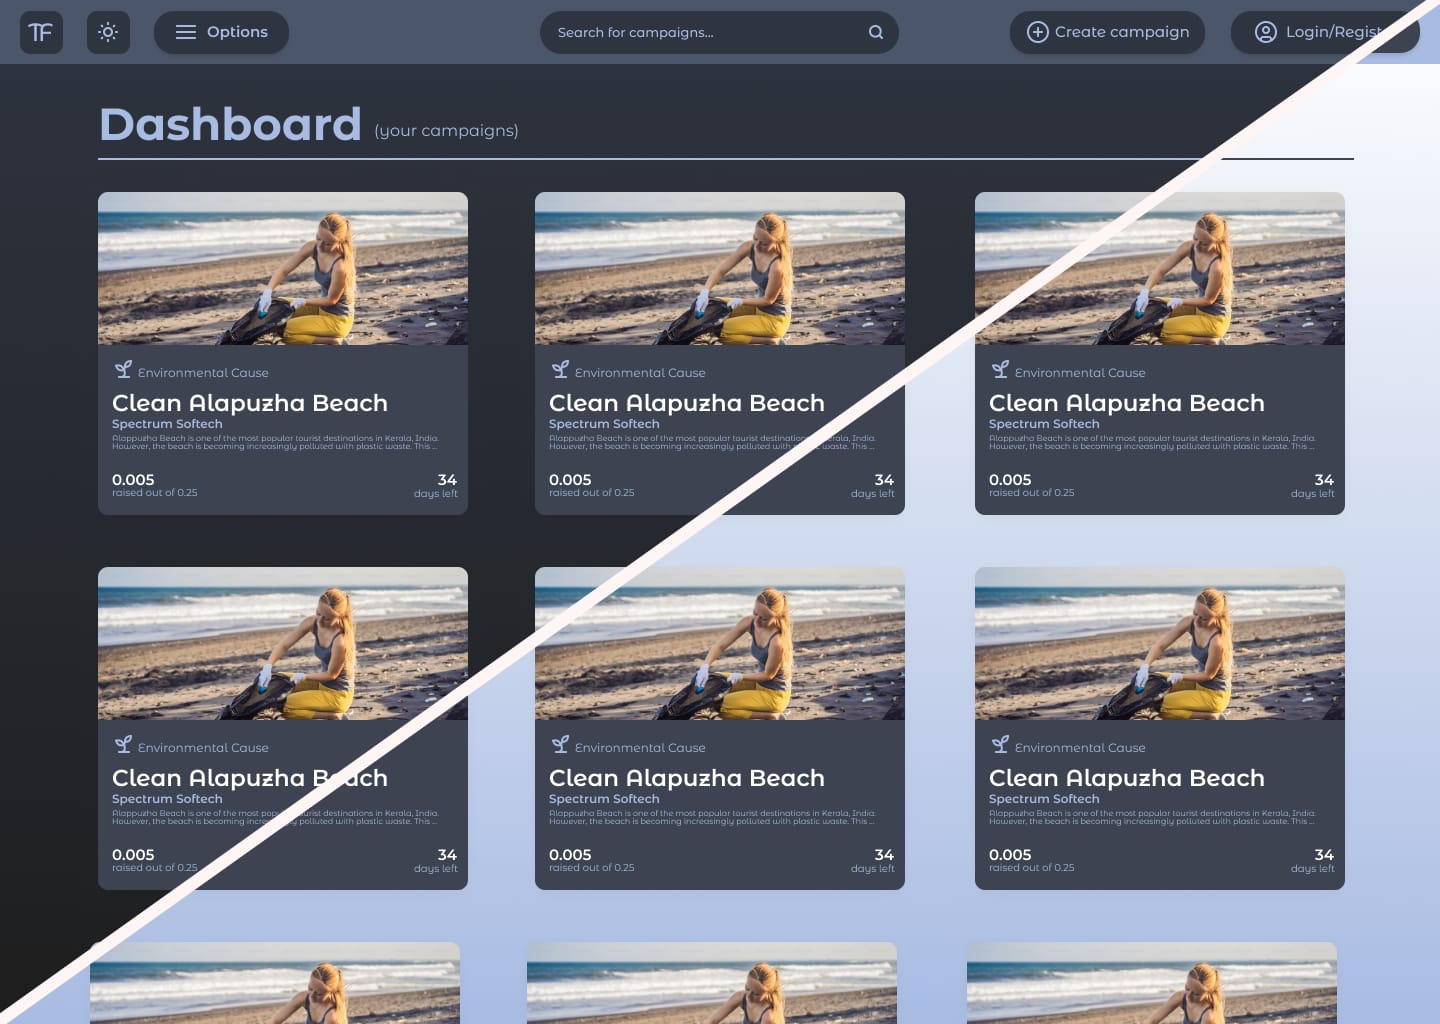
\includegraphics[width=\linewidth]{assets/ui/dashboard.jpeg} 
\end{frame}
\begin{frame}{Campaign Details}
    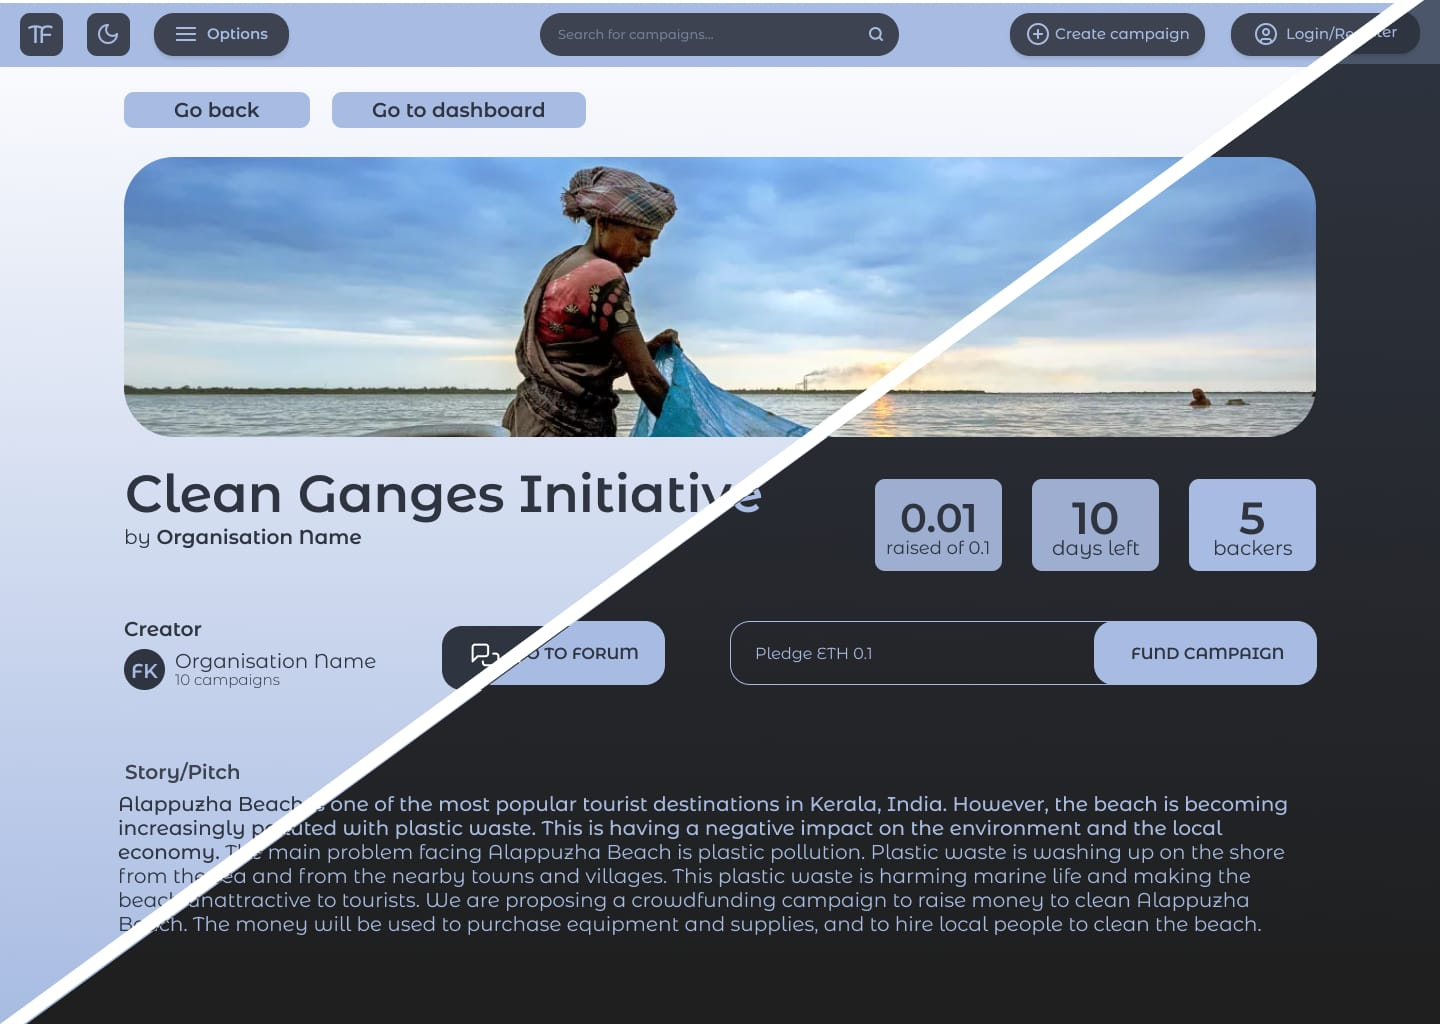
\includegraphics[width=\linewidth]{assets/ui/campaign-details.jpeg} 
\end{frame}
\begin{frame}{Create Campaign}
    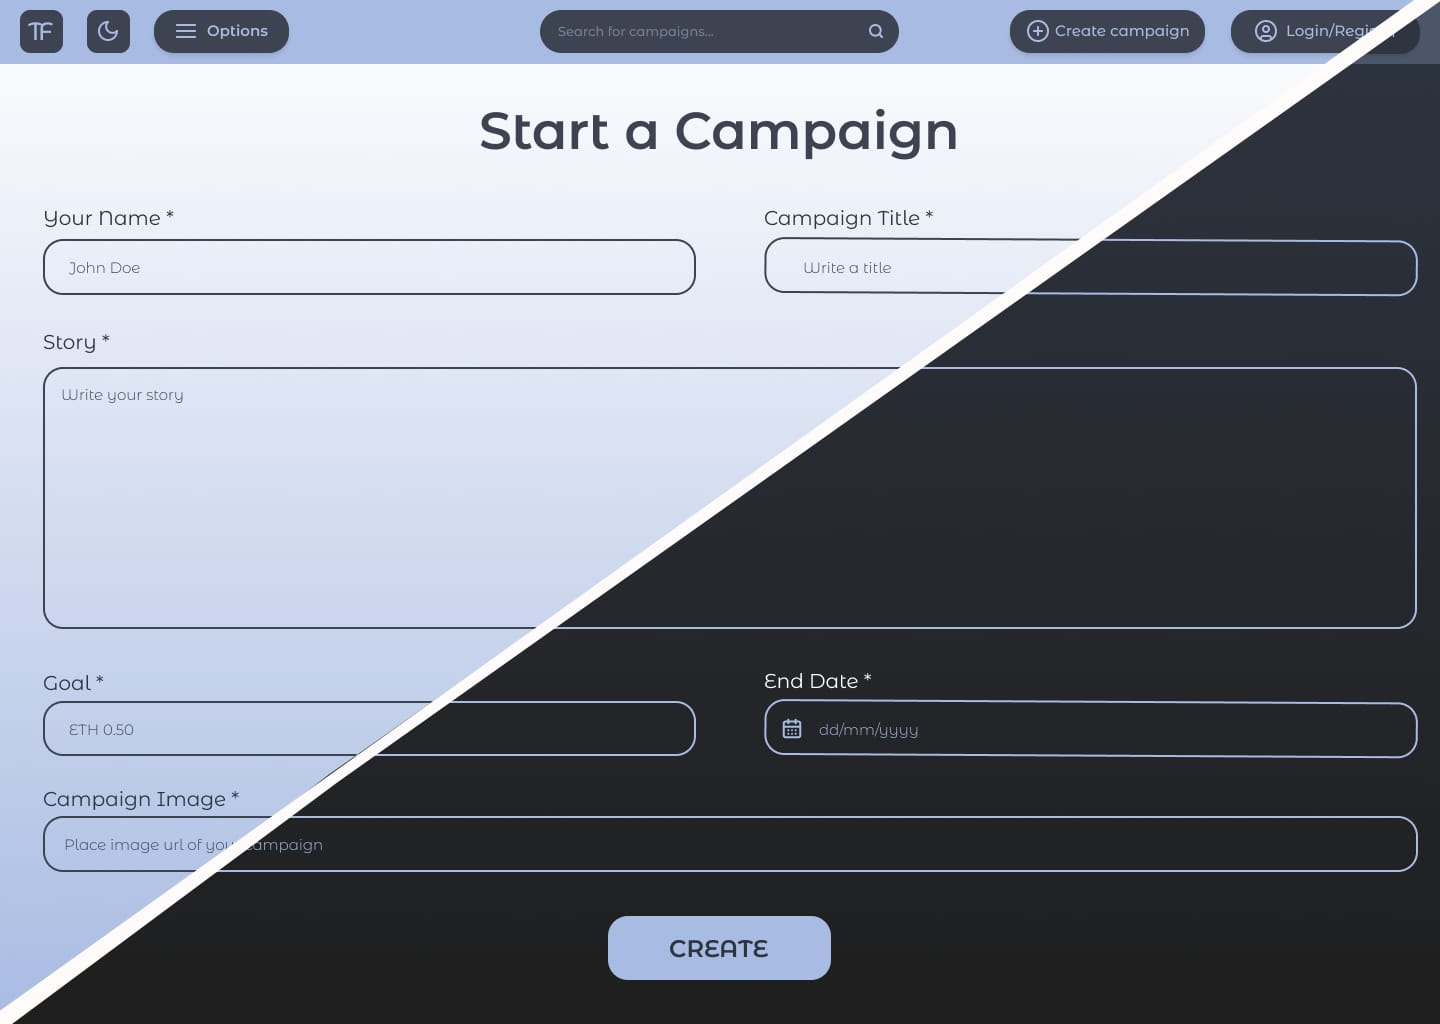
\includegraphics[width=\linewidth]{assets/ui/start-campaign.jpeg} 
\end{frame}


\section{Algorithms}
\begin{frame}{Registration - Algorithm}
  \setlength{\itemsep}{4pt}
   \begin{columns}[T]
        \begin{column}{0.55\textwidth}
        \fontsize{7}{9}\selectfont
        \begin{enumerate}
             \item Start
           \item  Receive registration request with user details 
            \item Check if User exists in Database
            \item If User exists, return a duplicate entry response
            \item Else check strength of password and complexity
            \item If Password is strong, proceed to next step
            \item Else return an error response
            \item Create User in Database with Verified Details and Password
            \item Route to the Login Page
            \item Stop
        \end{enumerate}
        \end{column}
        \begin{column}{0.6\textwidth}
            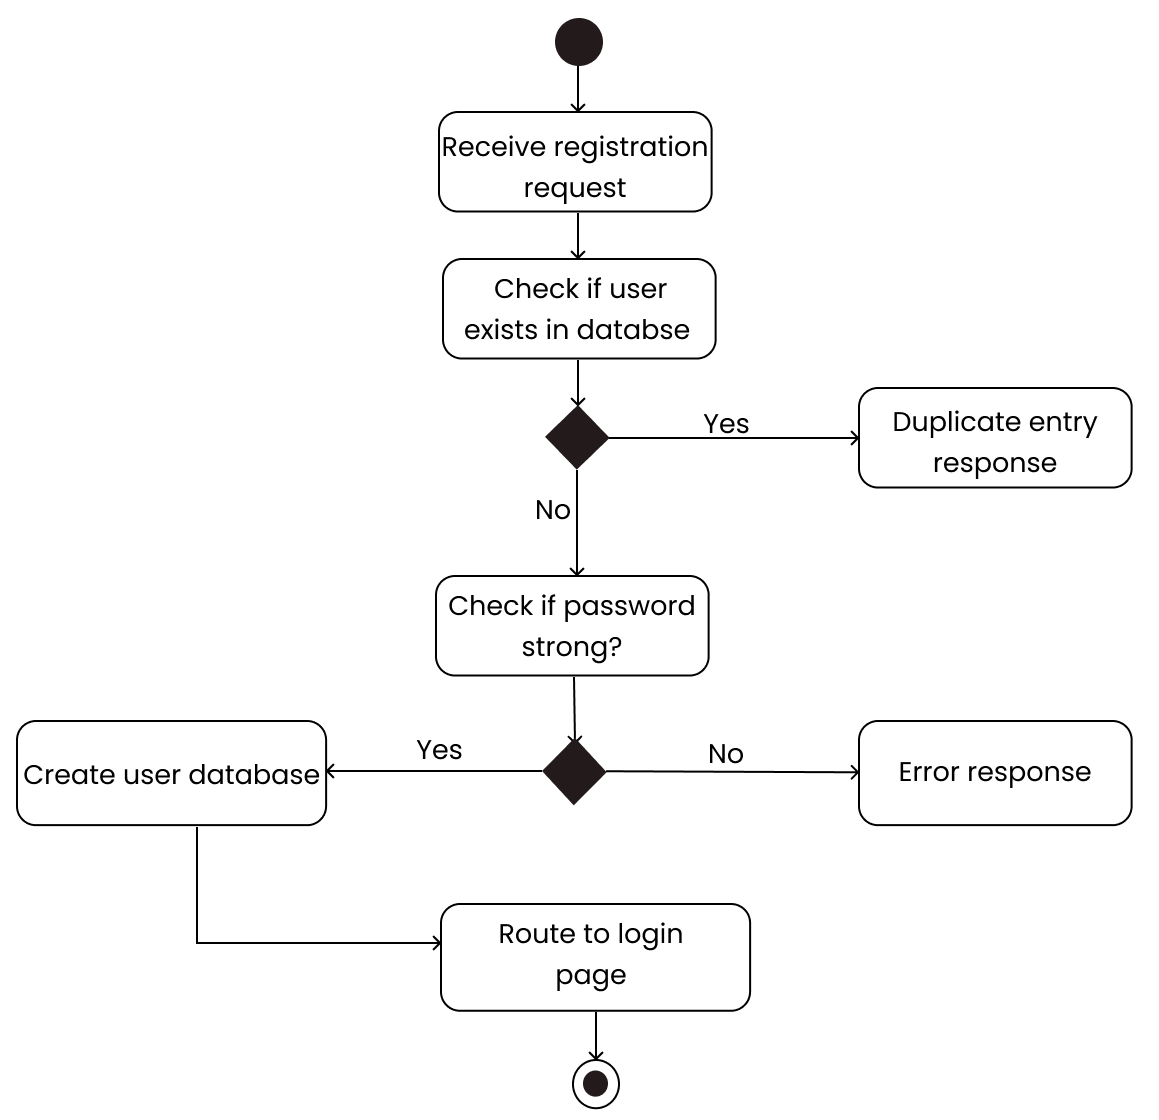
\includegraphics[width=\linewidth]{assets/Registration_state_chart.png} 
        \end{column}
    \end{columns}
    \end{frame}

  \begin{frame}{Login - Algorithm}
  \setlength{\itemsep}{4pt}
   \begin{columns}[T]
        \begin{column}{0.5\textwidth}
        \fontsize{7}{9}\selectfont
        \begin{enumerate}
            \item Start
            \item Receive login request with user credentials 
            \item Check if same user exists in the database
            \item Else return an authentication failure response
            \item Authenticate user password by comparing entered password with stored password
            \item If passwords match, go to next step
            \item Else return an authentication failure response
            \item Create a secure authentication token
            \item Associate the token with the user 
            \item Route to the User Dashboard or Home Page
            \item Stop
        \end{enumerate}
        \end{column}
        \begin{column}{0.6\textwidth}
            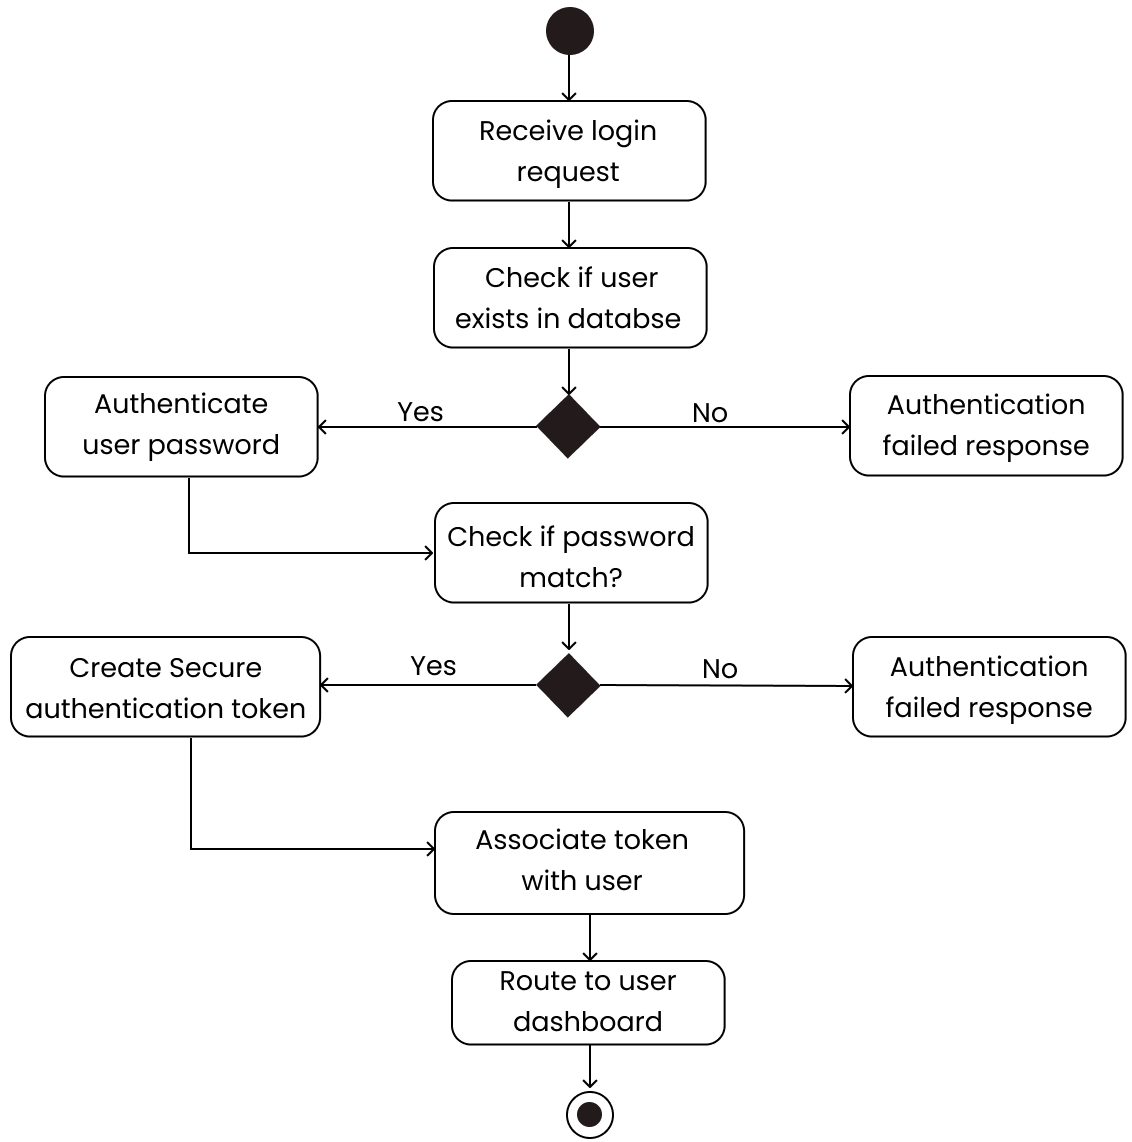
\includegraphics[width=\linewidth]{assets/login_state_chart.png} 
        \end{column}
    \end{columns}
    \end{frame}

     \begin{frame}{Create Campaign - Algorithm}
  \setlength{\itemsep}{4pt}
   \begin{columns}[T]
        \begin{column}{0.5\textwidth}
        \fontsize{7}{9}\selectfont
        \begin{enumerate}
             \item Start
            \item User initiates campaign creation
            \item Generate unique campaign identifier, use secure identifier generation 
            \item Frame a campaign smart contract 
            \item Specify parameters 
            \item Deploy campaign smart contract, confirm successful deployment
            \item Store campaign details on blockchain, record metadata
            \item Set campaign parameters allowing user parameter input
            
            \item Authorize campaign creator by confirming user identity 
            \item Set initial status then update blockchain with campaign status
            \item Stop
        \end{enumerate}
        \end{column}
        \begin{column}{0.6\textwidth}
          \vspace{20pt}
            \begin{center}
                 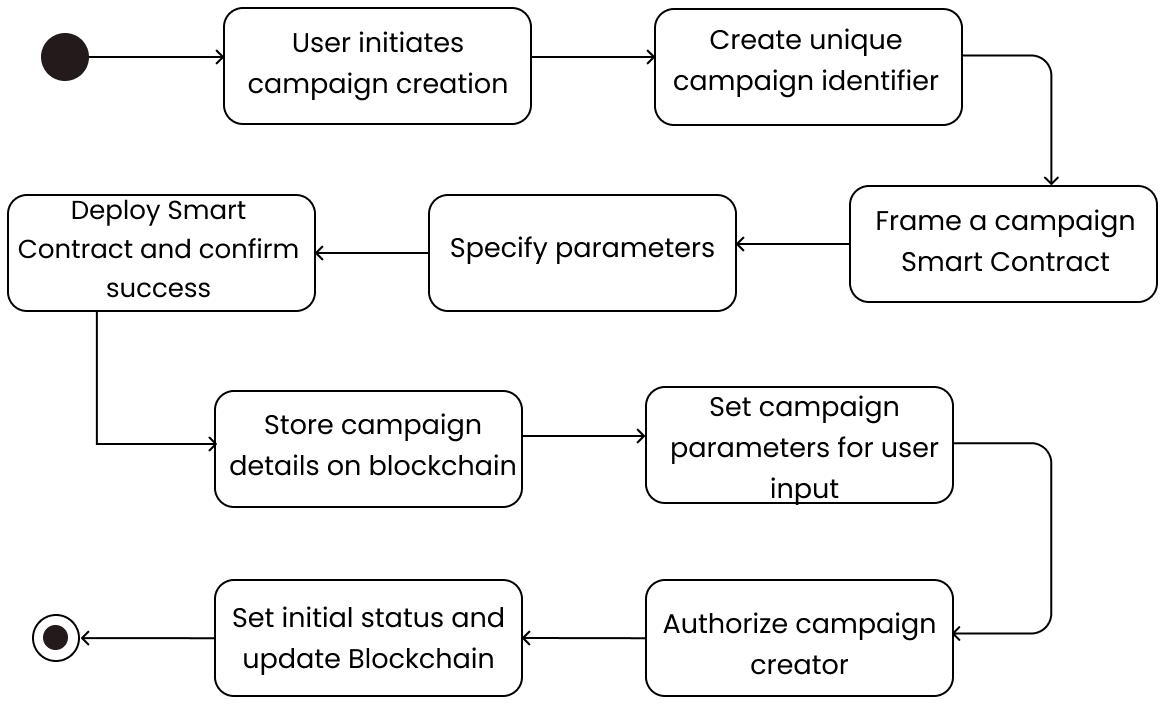
\includegraphics[width=\linewidth]{assets/campaign_creation_state_chart.png} 
            \end{center}
        \end{column}
    \end{columns}
    \end{frame}
    
  \begin{frame}{Campaign Donation - Algorithm}
   \begin{columns}[T]
        \begin{column}{0.53\textwidth}
        \fontsize{10}{12}\selectfont
        \begin{enumerate}
             \item Start
           \item User selects campaign to donate
           \item User initiates donation and authorisation is done
           \item Verify donation amount
           \item Retrieve campaign smart contract
           \item Contribute to the campaign and confirm user's contribution
           \item Update campaign balance
           \item Record donation details
           \item Stop
        \end{enumerate}
        \end{column}
        \begin{column}{0.73\textwidth}
            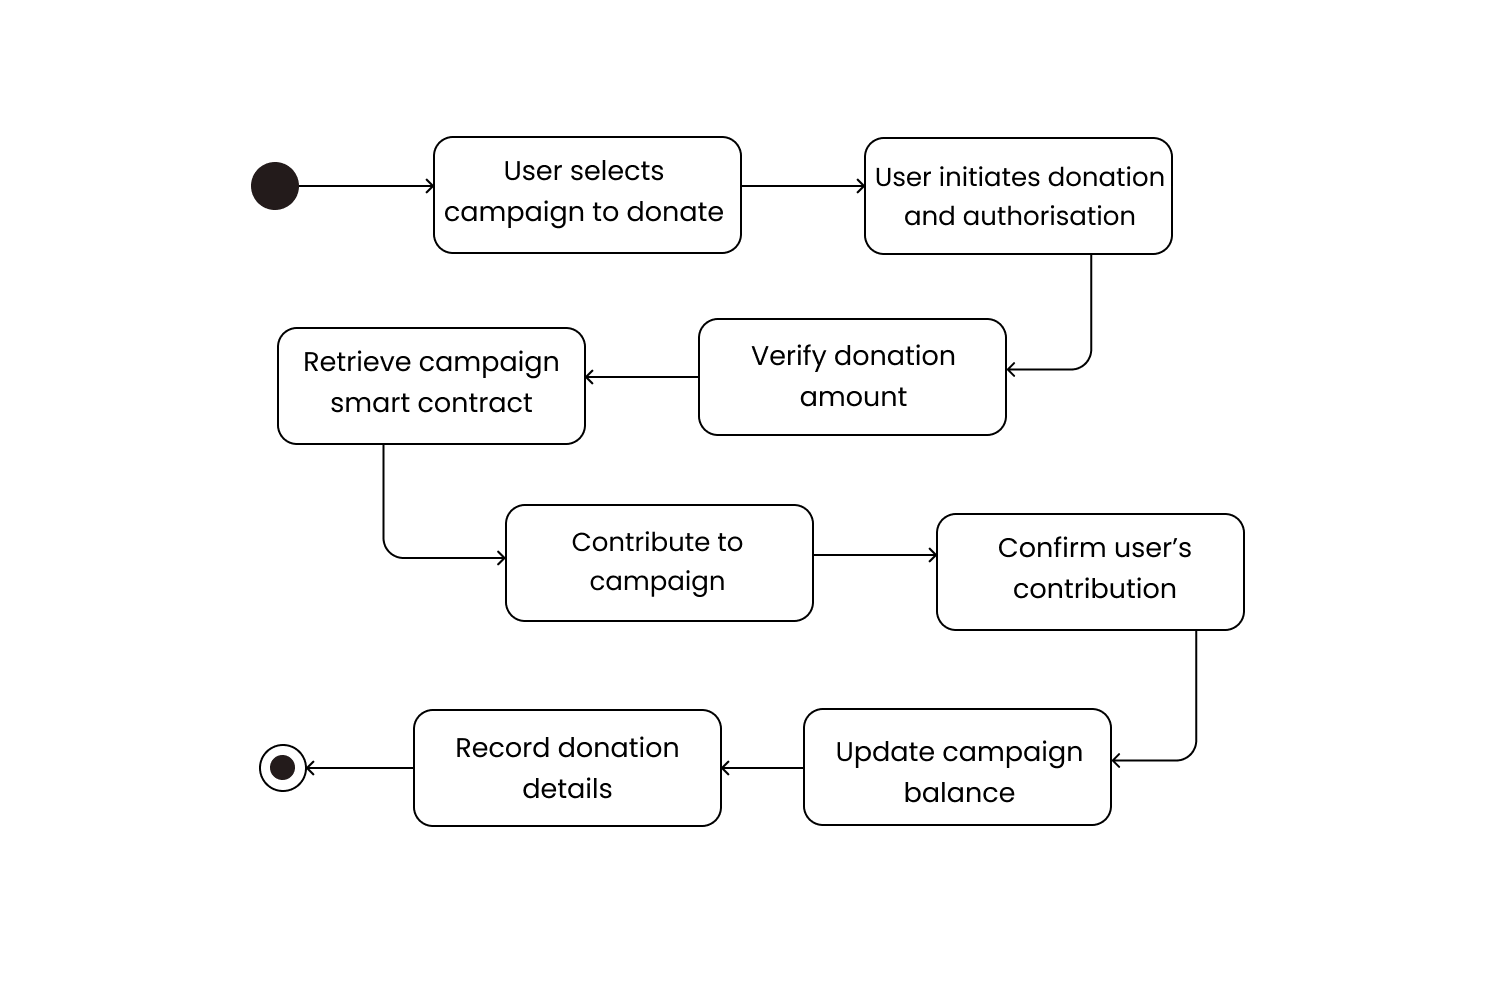
\includegraphics[width=\linewidth]{assets/donation_state_chart.png} 
        \end{column}
    \end{columns}
    \end{frame}

    
\begin{frame}{Explore Campaigns - Algorithm}
  \setlength{\itemsep}{4pt}
   \begin{columns}[T]
        \begin{column}{0.5\textwidth}
        \fontsize{10}{12}\selectfont
        \begin{enumerate}
              \item Start
            \item User accesses the home page which has explore campaign section.
            \item Display campaign details
            \item Paginate campaign results using infinite scrolling
            \item Clicking on a campaign would take it to its detail page
            \item Stop
        \end{enumerate}
        \end{column}
        \begin{column}{0.73\textwidth}
            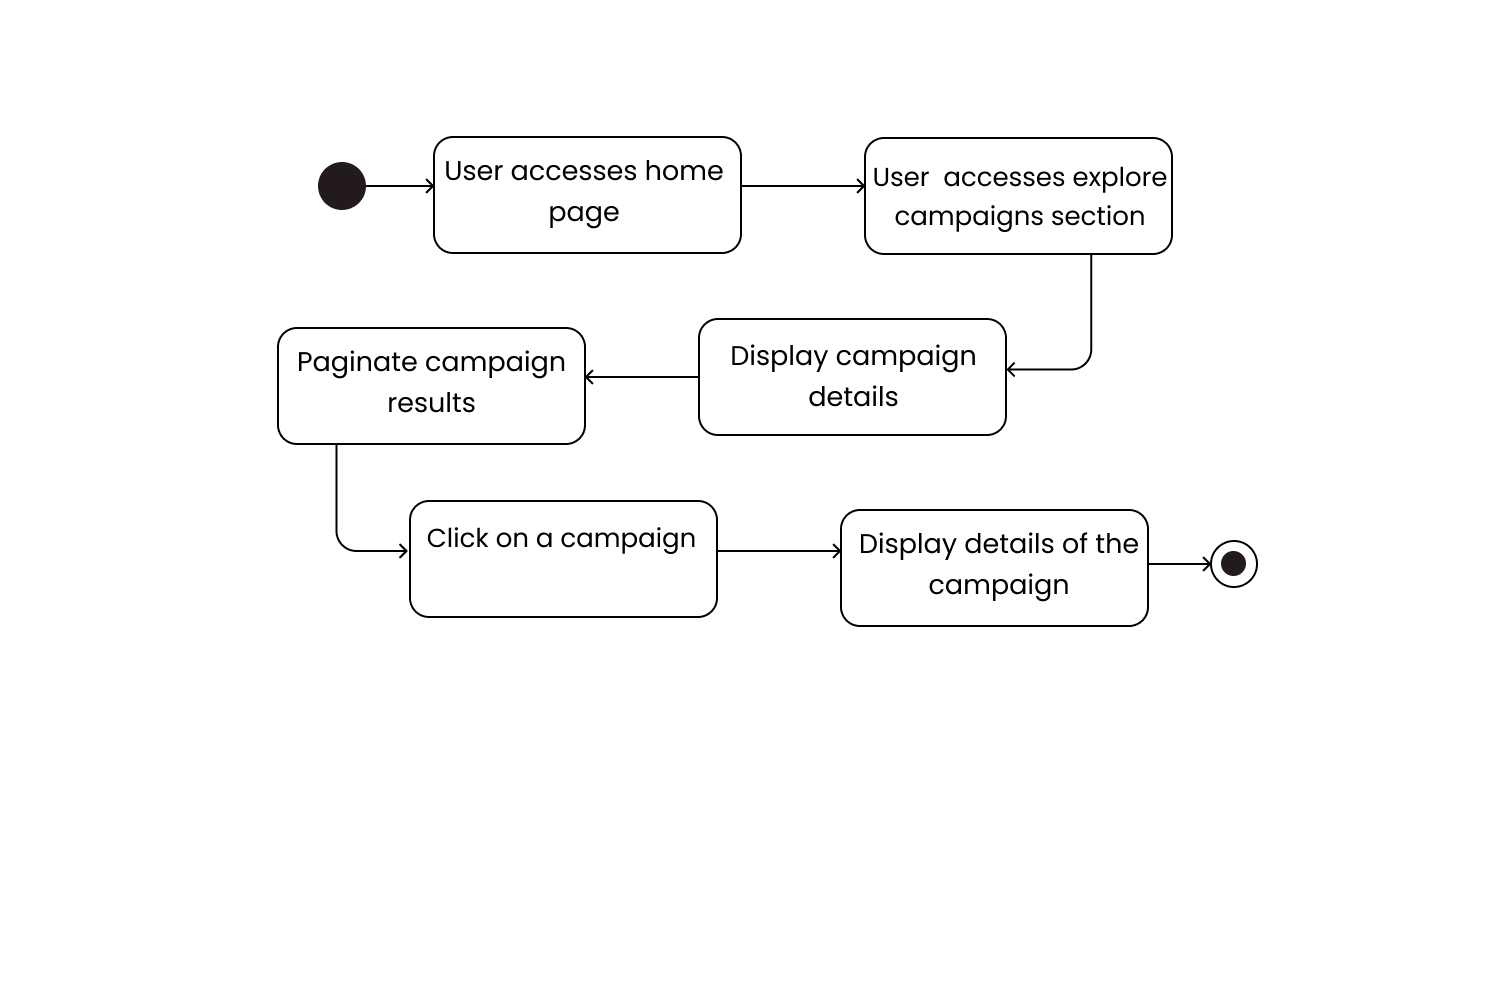
\includegraphics[width=\linewidth]{assets/explore_state_chart.png} 
        \end{column}
    \end{columns}
    \end{frame}


\begin{frame}{Campaign Forum - Algorithm}
  \setlength{\itemsep}{4pt}
   \begin{columns}[T]
        \begin{column}{0.48\textwidth}
        \fontsize{10}{12}\selectfont
        \begin{enumerate}
            \item Start
            \item Click on Campaign Forum Button in Campaign Detail page
            \item Display messages from the campaign creator, backers, public.
            \item Post messages by clicking on send button.
            \item Stop
        \end{enumerate}
        \end{column}
        \begin{column}{0.68\textwidth}
          \vspace{10pt}
            \begin{center}
                 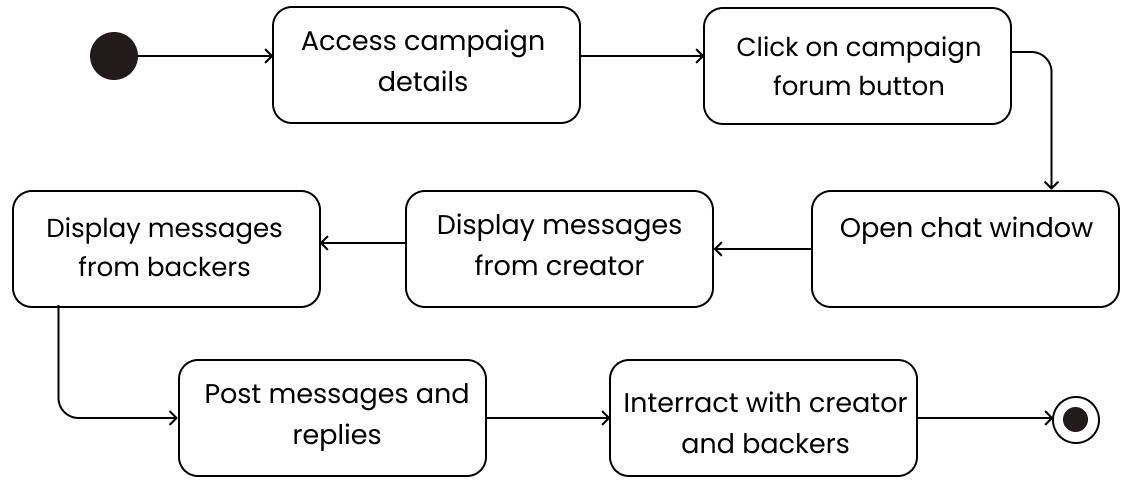
\includegraphics[width=\linewidth]{assets/forum_state_chart.png} 
            \end{center}
        \end{column}
    \end{columns}
    \end{frame}



\section{Database}
\begin{frame}{Database}
\hspace*{-1cm}
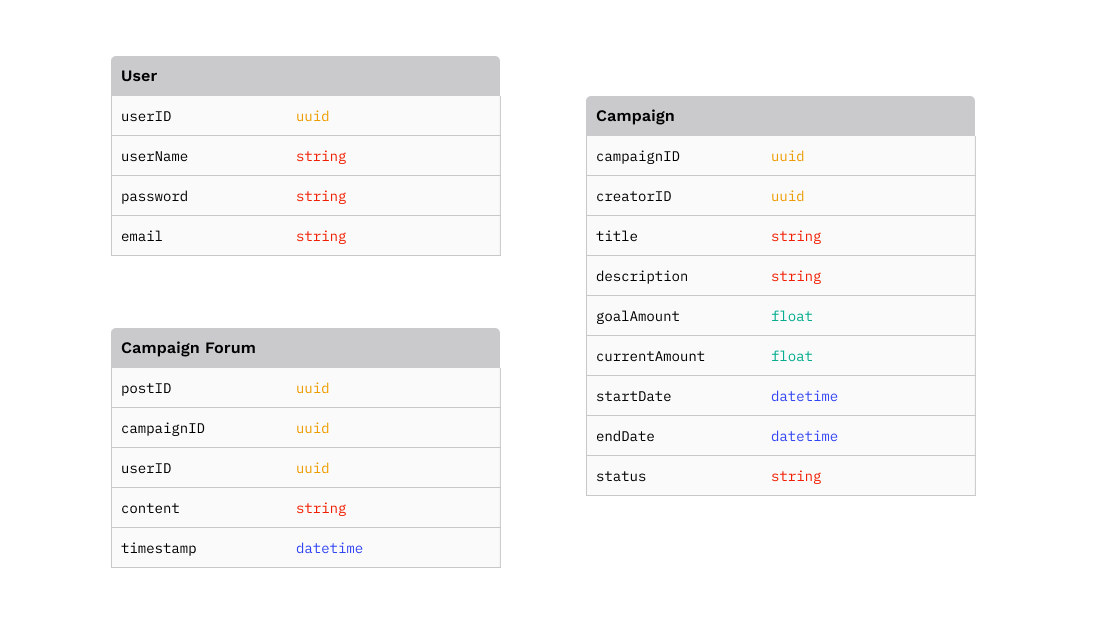
\includegraphics[width=1\paperwidth]{assets/Database.png}
\end{frame}

{\usebackgroundtemplate{
\includegraphics[width=\paperwidth,height=\paperheight]{assets/img1.png}}
\begin{frame}[plain]
  \centering
  \Huge{Thank You!}
\end{frame}
}

\end{document}

